\documentclass{article}
\usepackage[utf8]{inputenc}
\usepackage{graphicx}
\usepackage{url}
\usepackage{multirow}
\usepackage{array}
\usepackage{fancyhdr}
\usepackage[english]{babel}
\usepackage{wrapfig}
\usepackage{caption}
\usepackage{indentfirst}
\usepackage{geometry}
 \geometry{
 a4paper,
 total={170mm,257mm},
 left=20mm,
 top=20mm,
 }

\title{ProjectReport}

\date{\today}
\rfoot{Page \thepage}

\begin{document}

\maketitle

\begin{center}
% Table for group details begins
\begin{tabular}{|c|c|c|}
\hline 
Group Name & Roll Number & Name \\
\hline
\multirow{3}{*}{!dcOD'ed} & 140050064 & B Srinivas Naik \\
\cline{2-3}
 & 140050083 & KM Mugilvannan \\
 \cline{2-3}
 & 140050085 & Gowtham B \\
 \hline
\end{tabular}
% Table for group details ends
\end{center}

\newpage
\section*{Project Design}
\begin{figure}[h] 
\caption{Tom vs Jerry}
\begin{center}
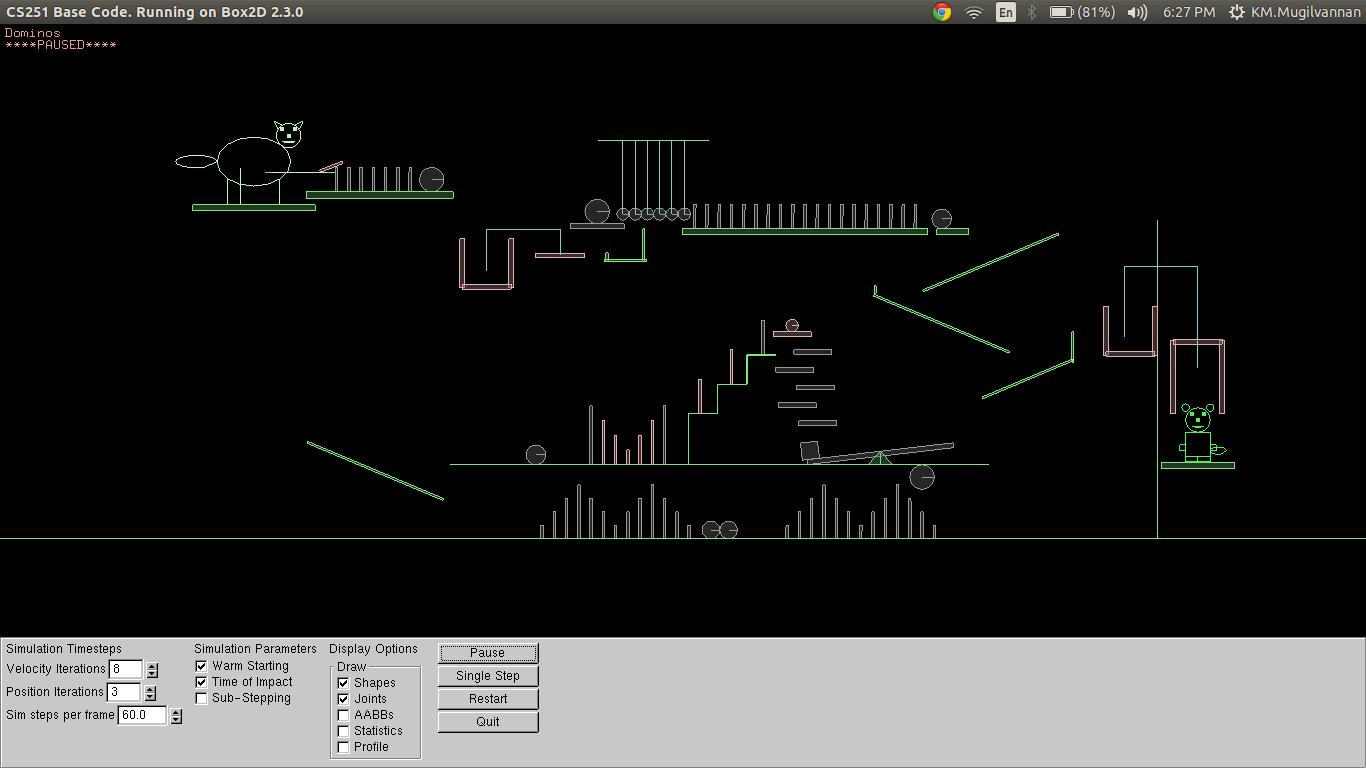
\includegraphics[height=8cm,scale=0.40]{Toms_turn}
\label{TomNjerry}
\end{center}
\end{figure}
%this is a floating image
\section*{Profile data} 
\begin{figure}[h] 
\caption{Profile picture}
\begin{center}
\includegraphics[height=6cm,width=18cm]{profile}
\label{profile}
\end{center}
\end{figure}


\newpage
\section{Title - Tom's Turn} \label{Title}
\section{Motivation} \label{Motivation} 
\subsection{Concepts learnt}
 The concepts learnt during the tenure of this project, we think, will help us learn concepts mentioned below and help us work in an actual software developing method which is GitHub.
\subsection{Tom and Jerry Rube Goldberg}
Tom tries to trap mouse but fails in its every attempt \cite{TomandJerry} . 
Now its Tom's turn..
\subsection{Size does NOT matter}
Being judgmental is not really a good thing. Never underestimate your opponent only because you think they are powerless. You may be wrong, after all!
\subsection{Be a team}
Yes, there would be endless fights between Tom and Jerry but they would make an effort to unite and stand up against their common enemy.
\subsection{Sharing is caring}
You always fight with those you sincerely care about. The bitter-sweet relationship of Tom and Jerry taught us why life is meaningless without a partner to share moments of fun and laughter with.
\subsection{Failure is the pillar of success}
Jerry, the smart mouse is an inspiration for all. He never surrenders, nor falls prey to Tom's traps. His intelligence and determination are enough to defeat the forever-conspiring cat. Never give up without trying!
\subsection{Be confident even in crisis}
Do not lose hope even at the gravest of situations. Stay strong!
\subsection{Don't let the spark disappear}
Celebrate what you have, dance and make merry. Worry less, let go and live for the moment. Carpe diem!

\section{Introduction} \label{Introduction}
    This project involves using the concepts of box2d to build the rube goldberg simulation which in our case is an interesting monologue between the famous disney characters tom and jerry. The difference in this version is that tom gets lucky by trapping jerry with a trap. The simulation starts with tom setting one of the dominos off balance and further following the simulation ends where the trap cage shuts jerry out of the outside. Here we have assumed that tom already knows the rat burrow which jerry uses as hidden route and uses ray casting to identify the length and time taken by jerry to reach the trap zone and thus setting the simulation accordingly.

\section{Bodyparts} \label{body}
    \subsection{Dominos}
        There are many places in the given simulation that dominos are used as element. These dominos are characterized by varying heights.
    \subsection{Pendulums}
        A series of pendulums are hung in the top part of the simulation to give variation on the type of physics elements used. As we know they follow the laws of Newton \cite{newton} perfectly if all the effects of nature i.e., friction, air drag, etc., are taken into account.
    \begin{figure}[h] 
    \caption{Simulation Screenshot involving pendulums and dominos}
    \begin{center}
    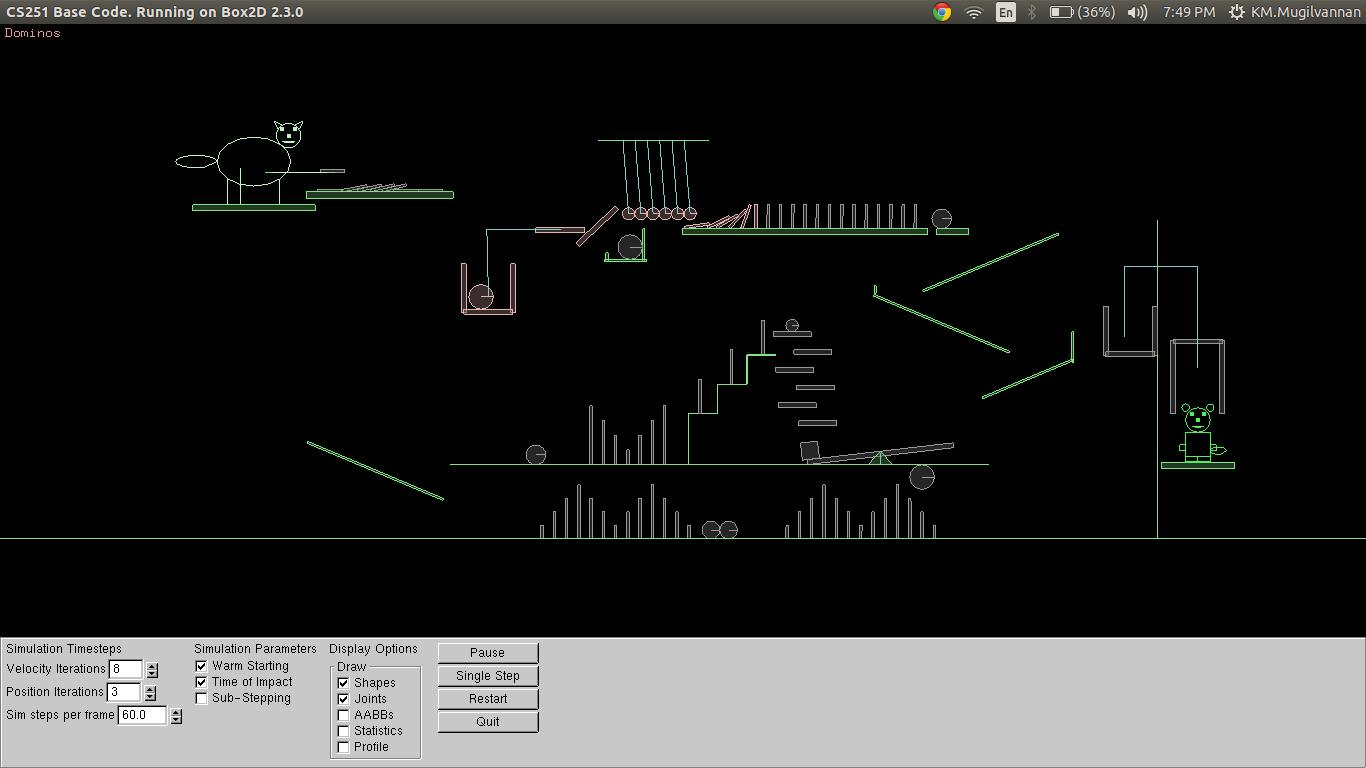
\includegraphics[height=8cm,scale=0.30]{Middle}
    \label{Intermediate simulation}
    \end{center}
    \end{figure}
    \subsection{Inclined Planes}
        A sequence of inclined planes are added to keep the simulation going and they follow they usual rules of opaque and dense bodies, except that they are fixed in their position.
    \subsection{Pulley systems}
        There are two places at which pulleys have been added to the simulation designed and they follow the Newton's laws \cite{newton} as well.    
    \subsection{Flyball}
        This ball is also a fantasy element used in the simulation which has the property of antigravity \cite{newton} 
    \begin{figure}[h] 
    \caption{Simulation screenshot involving the flying ball}
    \begin{center}
    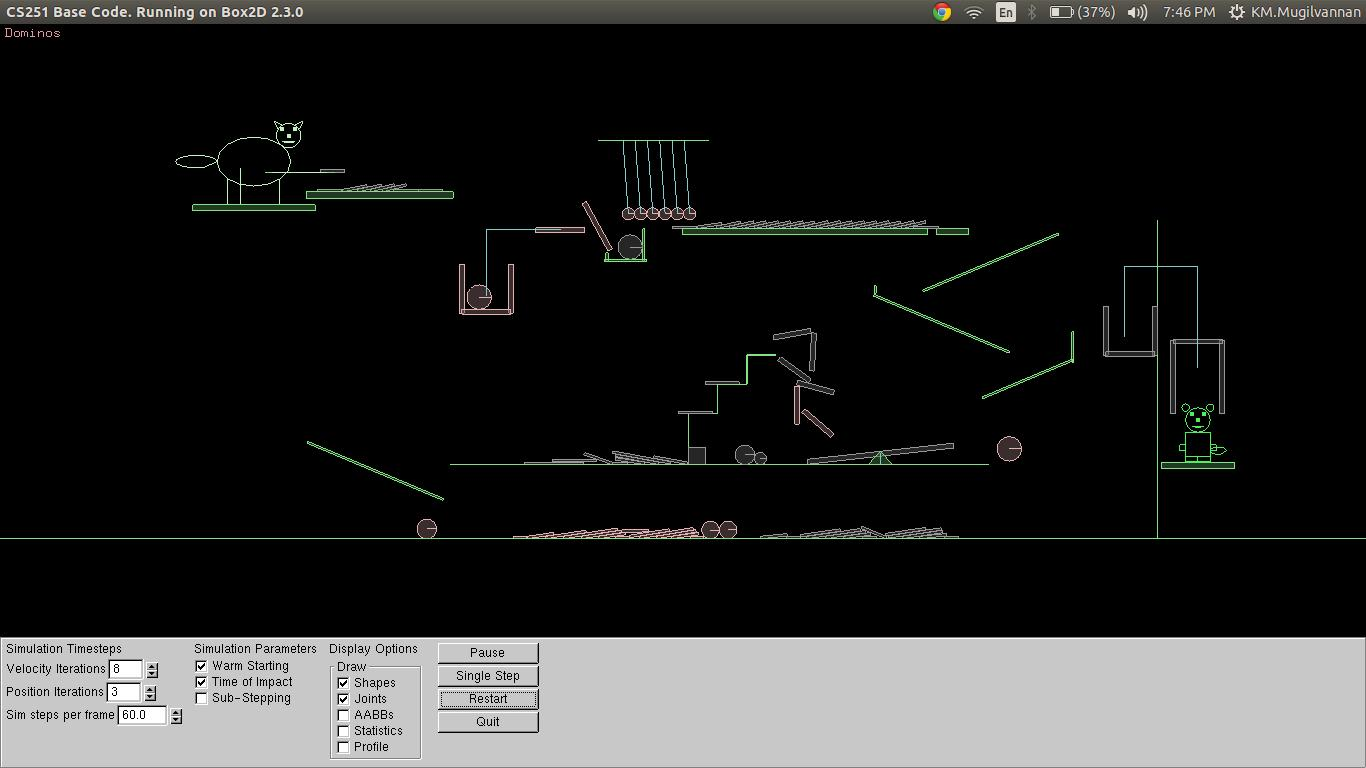
\includegraphics[height=8cm,scale=0.30]{Flyball}
    \label{Flying Ball}
    \end{center}
    \end{figure} 
    \subsection{Trap}
        Assuming that jerry had irritated tom and tom used ray casting  \cite{ray} techninique to identify jerry's usual path of escape, the trap here is used by Tom to catch Jerry when it tries to escape from Tom.  
    \begin{figure}[h] 
    \caption{Simulation screenshot involving involving the trap}
    \begin{center}
    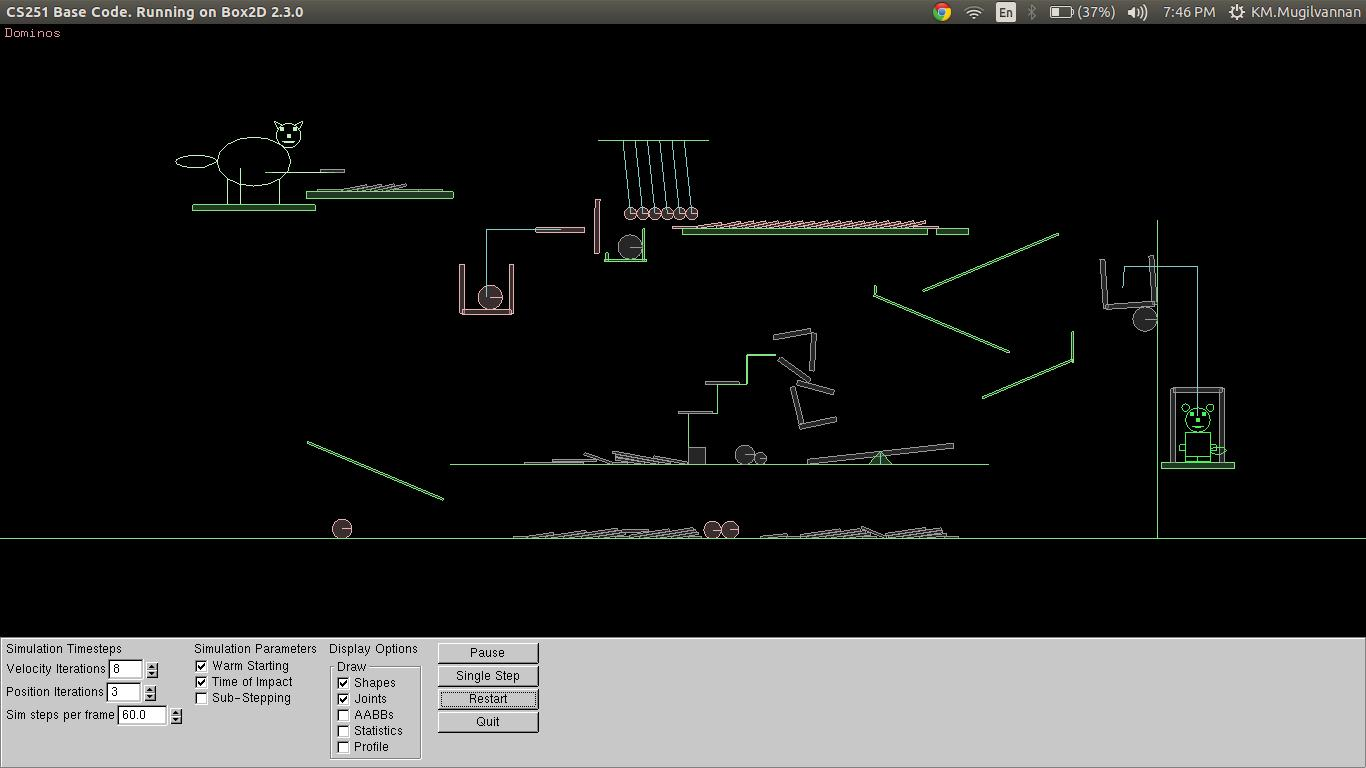
\includegraphics[height=8cm,scale=0.30]{Ending}
    \label{Flying Ball}
    \end{center}
    \end{figure}

\section{Deviations from Proposal}
    Some of the proposed items were difficult to be established and scraped off the simulation due to time constraint. They are
    \subsection{Conveyor Belt}
        The  implementation of conveyer belt needed the PreSolve function of the ContactListener class to be modified in the child class inherited from it to override the basic definition. But even after modifying the function both in the base\_sim\_t child class of ContactListener and dominos\_t child class of base\_sim\_t, the intended action was not acquired. Various strategies planned didn't help which led to dropping the idea.
    \subsection{Boat}
    \subsection{Wheel}
        The concept of wheel was replaced with Conveyor belt, so it was not implemented.
    \subsection{Difficulties faced}
        \subsubsection{Working on GitHub}
            Initial working on the Git repositories was difficult since we were used to sending mails and messaging in facebook. But with time, practice and motivation towards its importance in the software development sector, we were up and running with coped measures to avoid those difficulties.  
        \subsubsection{Time of discussion}
            Finding quality time of discussion off the inlabs and outlabs with group peers was difficult, because of the modes of communication preferred by the members of the team
        \subsubsection{Splitting of Work}
            Dividing the work amongst each member in the team to keep everyone on the same page with each having equal precentage of work distribution was a hurdle to cross through 

\section{Areas of contribution}
    \textbf{B Srinivas} - Box2d code for the dominos, tom and jerry designs, flying ball \cite{box2d}, inclined planes, Project webpage \newline
    \indent \textbf{KM Mugilvannan} - Box2d code for conveyor belt \cite{box2d}, Project report, Project presentation, Makefile, Project webpage \newline 
    \indent \textbf{B Gowtham} - Box2d code for dominos, inclined plane, flying ball, boat \cite{box2d} \newline  

\section{Conclusion} \label{Conclusion}
    Learning concepts like
    \subsection{Make}
    \subsection{makefiles}
    \subsection{cmake}
    \subsection{Box2D simulation}
    \subsection{Analysis of Dominos}
    \subsection{Profiling and Debugging Errors}
    \subsection{GitHub}
    \subsection{Referral and Analysis of projects of seniors \cite{saikiran} \cite{amangoel}} 
    \subsection{Learning basic concepts of \LaTeX}
    \subsection{Physics in General}

\section{Honor Codes} \label{Honor Codes}
    \textbf{B.Srinivas Naik,140050064} \% contribution = 100 \newline
    \indent\indent I pledge on my Gita that I have not given or received any unauthorized assistance on this assignment or any previous task. \newline
    \indent \textbf{KM.Mugilvannan,140050083} \% contribution = 100 \newline 
    \indent\indent I pledge on my Gita that I have not given or received any unauthorized assistance on this assignment or any previous task.\newline 
    \indent \textbf{B.Gowtham,140050085} \% contribution = 100 \newline
    \indent\indent I pledge on my Gita that I have not given or received any unauthorized assistance on this assignment or any previous task.

\bibliographystyle{unsrt}%Used BibTeX style is unsrt
\bibliography{ProjectProposal}   
\end{document}
